\chapter{Simulação}
\section{Objetivo}

O objetivo da simulação é poder realizar teste em ambiente controlado, de forma a se averiguar a precisão, acurácia e velocidade de processamento da posição por parte do Star Tracker. Para isto, a simulação deve implementar modelos matemáticos que representem o sistema real o mais fielmente possível.

\section{Recursos e características}

\textbf{GUI (Graphical User Interface):} A simulação é inteiramente controlada através de uma GUI criada para facilitar o controle e a execução dos testes, também é utilizada para facilitar a visualização e a correção de possíveis erros e bugs no software e no desenvolvimento do trabalho em geral. A implementação dos módulos de funcionamento do software segue conceitos dos TDD (Test driven  development), juntamente da arquitetura de software MVC (model view controller), para organizar o funcionamento da interface em si.

\textbf{Gerador de campo de visão:} Esta é a função principal do software de simulação, que é gerar uma janela com o campo de visão que teoricamente seria visto pela câmera, a imagem gerada é monocromática com as estrelas projetadas sobre a superfície plana do monitor, neste trabalho as estrelas simuladas são apenas círculos brancos em um fundo preto, porém são estrelas retiradas de uma base de dados reais.

\textbf{Load de arquivos:} Para facilitar a mudança de parâmetros durante os testes e simulações , o software carrega todas as informações inerentes a configuração e execução dos testes, através de caixas de diálogo que pedem a seleção dos arquivos de simulação. Para uma maior modularidade, cada informação está dividida em arquivos diferentes, com arquivos separados para configuração de câmera, base de dados de estrelas e sequência de movimentos a ser realizada.

\textbf{Elementos auxiliares de visualização:} Além das funcionalidades básicas, o software implementa  recursos de configuração  de aspectos visuais. Apesar de não serem estritamente necessários são de extrema importância  para análises menos rigorosas das informações, como por exemplo, o plot 3D, a projeção cartográfica em 2D. Com opções de visualização da posição das câmeras e demais auxílios.

\textbf{Controles manuais e automáticos:} O software possui controles manuais de rotação, que permitem a rotação da simulação em todos os 3 eixos de liberdade, através de configurações na GUI, além disto o usuário pode preparar uma sequência de movimentos e suas respectivas durações previamente.

\textbf{Salvar frames:} O usuário pode salvar frames de imagem em arquivos png para facilitar a utilização posterior da posição.

\section{Projeção em perspectiva}

A projeção descreve matemática como representar um ponto com 3 graus de liberdade, no espaço bidimensional do monitor e do frame da câmera. Essa transformação pode ser realizada através de matrizes, que levam em consideração elementos como o ângulo focal da lente, a resolução e proporção da imagem.

\subsection{Square Frustum}

Frustum retangular é um espaço que contém a linha de visão de  um visualizador como se este possuísse um ângulo de visão retangular, que é caso de câmeras com CCD retangulares, para melhor entender este conceito recomenda-se a observação da Figura \ref{fig:frustum}.

\begin{figure}[h]
    \centering
    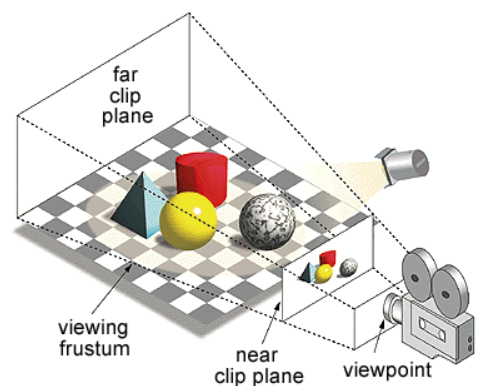
\includegraphics[width=0.5\textwidth]{images/frustum.png}
    \caption{Visualização Frustum rectangular, Fonte: ~\cite[]{the_free_dictionary}}
    \label{fig:frustum}
\end{figure}

A existência de um plano ao fundo na cena (far clip), se deve ao equacionamento que leva os pontos presentes na cena 3D para o frame 2D da câmara, além de reduzir o custo de processamento requerido pelo programa para gerar a cena sendo parte importante do equacionamento do frame da câmera.

Considerando que o ângulo de visão da câmera esteja apontada para o positivo do eixo x como é mostrado na figura \ref{fig:posicao_inicial_camera}.

\begin{figure}[h]
    \centering
    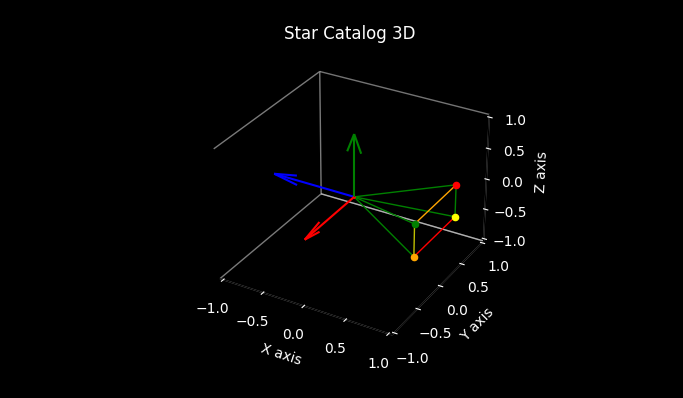
\includegraphics[width=0.5\textwidth]{images/posicao_inicial_camera.png}
    \caption{Visualização da câmera na posição inicial}
    \label{fig:posicao_inicial_camera}
\end{figure}

As setas coloridas presentes na imagem são as coordenadas do frame da câmera, que seguem um esquema de cores usual para esse tipo de aplicação, na figura 17 é demonstrado as relações X,Y e Z com as cores:



\begin{figure}[h]
    \centering
    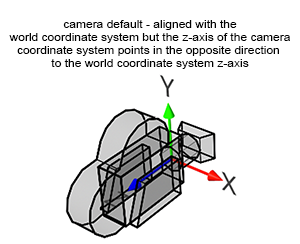
\includegraphics[width=0.5\textwidth]{images/coordenadas.png}
    \caption{Coordenadas do frame da camera. Fonte: ~\cite[]{the_free_dictionary}}
    \label{fig:coordenadas}
\end{figure}


Com isso se desenvolveu a seguinte equação matricial da câmera, seguindo os passos mostrados por Brendan Galea em seu video ~\cite[]{Galea}:

\begin{equation}
    \begin{bmatrix}
        x' \\
        y' \\
        z' \\
        w
    \end{bmatrix}
    =
    \begin{bmatrix}
        \frac{f+n}{f-n} & 0                                 & 0                               & \frac{-2fn}{f-n} \\
        0               & \frac{h}{w*tan(\frac{\theta}{2})} & 0                               & 0                \\
        0               & 0                                 & \frac{1}{tan(\frac{\theta}{2})} & 0                \\
        1               & 0                                 & 0                               & 0
    \end{bmatrix}
    \begin{bmatrix}
        x \\
        y \\
        z \\
        1
    \end{bmatrix}
\end{equation}

Em que, \textbf{f} é a distância do far plane ao ponto (0,0,0), que neste caso é sempre unitário já que a estrelas estão presentes em um círculo unitário, $\Theta$ é o ângulo de abertura  da câmera, \textbf{w} é a quantidade de pixels na horizontal camera, \textbf{h} é quatidade e pixel na vertical da câmera por fim \textbf{n} é a distância do near plane, que neste caso é o coseno de $\frac{\Theta}{2}$.

Nota-se que a matriz de transformação da câmera é uma matriz 4X4 isso ocorre pois as equações de transformação são realizadas através de coordenadas homogêneas e não coordenadas cartesianas tradicionais.

Além da matriz, existe uma equação de clipping que determina se uma estrela deve ou não aparecer no frame, devido a simplicidade da simulação aqui implementada essa equação se tornou apenas um cheque se a estrela se encontrava na metade da esfera celeste em que x é positivo.

O resultado dessa simulação pode ser visto na Figura \ref{fig:resultado_simulacao}.

\begin{figure}[h]
    \centering
    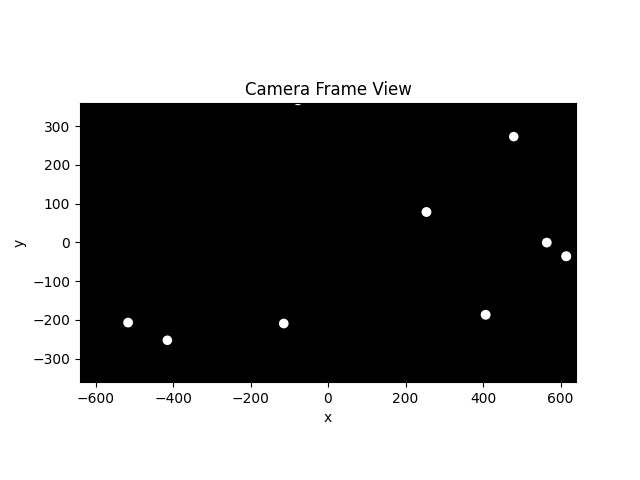
\includegraphics[width=\textwidth]{images/resultado_simulacao.png}
    \caption{Camera frame at position,declination 0º, arcensão 0º, roll 0º}
    \label{fig:resultado_simulacao}
\end{figure}